\chapter{Icon Language Overview}

\textsc{Perspective}: The implementer of a programming language needs
a considerably different understanding of the language from the
persons who are going to use it. An implementer must have a deep
understanding of the relationships that exist among various aspects of
the language and a precise knowledge of what each operation
means. Special cases and details often are of particular importance to
the implementer. Users of a language, on the other hand, must know how
to use features to accomplish desired results. They often can get by
with a superficial knowledge of the language, and they often can use
it effectively even if some aspects of the language are
misunderstood. Users can ignore parts of the language that they do not
need. Idiosyncrasies that plague the implementer may never be
encountered by users.  Conversely, a detail the implementer overlooks
may bedevil users. Furthermore, the implementer may also need to
anticipate ways in which users may apply some language features in
inefficient and inappropriate ways.

Part I of this book is about the implementation of Version 6
(discussion partially updated to Version 9) of Icon. The description
that follows concentrates on aspects of the language that are needed
to understand its implementation. Where there are several similar
operations or where the operations are similar to those in well-known
programming languages, only representative cases or highlights are
given. A complete description of Icon for the user is contained in
Griswold and Griswold (1997).

Icon is an unusual programming language, and its unusual features are
what make its implementation challenging and interesting. The
interesting features are semantic, not syntactic; they are part of
what the language can do, not part of its appearance. Syntactic
matters and the way they are handled in the implementation are of
little interest here.  The description that follows indicates syntax
mostly by example.

This chapter is divided into two major parts. The first part describes
the essential aspects of Icon. The second part discusses those aspects
of Icon that present the most difficult implementation problems and
that affect the nature of the implementation in the most significant
ways.

\section{The Icon Programming Language}

Icon is conventional in many respects. It is an imperative, procedural
language with variables, operations, functions, and conventional data
types. Its novel aspects lie in its emphasis on the manipulation of
strings and structures and in its expression-evaluation
mechanism. While much of the execution of an Icon program has an
imperative flavor, there also are aspects of logic programming.

There are no type declarations in Icon. Instead, variables can have
any type of value. Structures may be heterogeneous, with different
elements having values of different types. Type checking is performed
during program execution, and automatic type conversion is
provided. Several operations are polymorphic, performing different
operations depending on the types of their arguments.

Strings and structures are created during program execution, instead
of being declared and allocated during compilation.  Structures have
pointer semantics; a structure value is a pointer to an object.
Storage management is automatic. Memory is allocated as required, and
garbage collection is performed when necessary. Except for the
practical considerations of computer architecture and the amount of
available memory, there are no limitations on the sizes of objects.

An Icon program consists of a series of declarations for procedures,
records, and global identifiers. Icon has no block structure. Scoping
is static: identifiers either are global or are local to procedures.

Icon is an expression-based language with reserved-word syntax. It
resembles C in appearance, for example (Kernighan and Ritchie 1978).

{\sffamily\bfseries
2.1.1 Data Types}

Icon has many types of data --- including several that are not found in
most programming languages. In addition to the usual integers and real
(floating-point) numbers, there are strings of characters and sets of
characters (csets). There is no character data type, and strings of
characters are data objects in their own right, not arrays of
characters.

There are four structure data types that comprise aggregates of
values: lists, sets, tables, and records. Lists provide positional
access (like vectors), but they also can be manipulated like stacks
and queues. Sets are unordered collections of values on which the
usual set operations can be performed. Tables can be subscripted with
any kind of value and provide an associative-access mechanism. Records
are aggregates of values that can be referenced by name.  Record types
also add to the built-in type repertoire of Icon.

The null value serves a special purpose; all variables have the null value initially. The null value is illegal in most
computational contexts, but it serves to indicate default values in a number of situations. The keyword \&null produces
the null value.

A source-language file is a data value that provides an interface
between the program and a data file in the environment in which the
program executes.

Procedures also are data values --- {\textquotedbl}first-class data
objects{\textquotedbl} in LISP parlance.  Procedures can be assigned
to variables, transmitted to and returned from functions, and so
forth. There is no method for creating procedures during program
execution, however.

Finally, there is a co-expression data type. Co-expressions are the
expression-level analog of coroutines. The importance of
co-expressions is derived from Icon's expression-evaluation mechanism.

Icon has various operations on different types of data. Some
operations are polymorphic and accept arguments of different
types. For example, type(x) produces a string corresponding to the
type of x. Similarly, copy(x) produces a copy of x, regardless of its
type. Other operations only apply to certain types. An example is:

{\ttfamily\mdseries
\ \ \ *x}


\noindent which produces the size of x, where the value of x may be a
string, a structure, and so on. Another example is ?x, which produces
a randomly selected integer between 1 and x, if x is an integer, but a
randomly selected one-character substring of x if x is a string, and
so on. In other cases, different operations for similar kinds of
computations are syntactically distinguished. For example,

{\ttfamily\mdseries
\ \ \ i = j}

\noindent compares the numeric values of i and j, while

{\ttfamily\mdseries
\ \ \ s1 == s2}


\noindent compares the string values of s1 and s2. There is also a
general comparison operation that determines whether any two objects
are the same:

{\ttfamily\mdseries
\ \ x1 === x2}

As mentioned previously, any kind of value can be assigned to any
variable. For example, x might have an integer value at one time and a
string value at another:

{\ttfamily\mdseries
\ \ \ x := 3 \\
\ \ \ ... \\
\ \ \ x := {\textquotedbl}hello{\textquotedbl}}

Type checking is performed during program execution. For example, in

{\ttfamily\mdseries
\ \ \ i := x + 1}

the value of x is checked to be sure that it is numeric. If it is not
numeric, an attempt is made to convert it to a numeric type. If the
conversion cannot be performed, program execution is terminated with
an error message.

Various conversions are supported. For example, a number always can be
converted to a string. Thus,

{\ttfamily\mdseries
\ \ \ write(*s)}

\noindent automatically converts the integer returned by *s to a
string for the purpose of output.

There also are explicit type-conversion functions. For example,

{\ttfamily\mdseries
\ \ \ s1 := string(*s2)}

\noindent assigns to s1 a string corresponding to the size of s2.

A string can be converted to a number if it has the syntax of a number. Thus,

{\ttfamily\mdseries
\ \ \ i := i + {\textquotedbl}20{\textquotedbl}}

\noindent produces the same result as

{\ttfamily\mdseries
\ \ \ i := i + 20}


Augmented assignments are provided for binary operations such as the
previous one, where assignment is made to the same variable that
appears as the left argument of the operation. Therefore, the previous
expression can be written more concisely as

{\ttfamily\mdseries
\ \ \ i +:= 20}


Icon also has the concept of a numeric type, which can be either an
integer or a real (floating-point) number.

{\sffamily\bfseries
2.1.2 Expression Evaluation}


In most programming languages --- Algol, Pascal, PL/I, and C, for
example --- the evaluation of an expression always produces exactly
one result. In Icon, the evaluation of an expression may produce a
single result, it may produce no result at all, or it may produce a
sequence of results.

\textbf{Success and Failure}. Conventional operations in Icon
produce one result, as they do in most programming languages. For
example,

{\ttfamily\mdseries
\ \ \ i + j}

\noindent produces a single result, the sum of the values of i and
j. However, a comparison operation such as

{\ttfamily\mdseries
\ \ \ i {\textgreater} j}

\noindent produces a result (the value of j) if the value of i is
greater than the value of j but does not produce a result if the value
of i is not greater than j.

An expression that does not produce a result is said to \textit{fail},
while an expression that produces a result is said to
\textit{succeed}. Success and failure are used in several control
structures to control program flow. For example,

{\ttfamily\mdseries
\ \ \ if i {\textgreater} j then write(i) else write(j)}

\noindent writes the maximum of i and j. Note that comparison
operations do not produce Boolean values and that Boolean values are
not used to drive control structures. Indeed, Icon has no Boolean
type.

Generally speaking, an operation that cannot perform a computation
does not produce a result, and hence it fails. For example,
type-conversion functions fail if the conversion cannot be
performed. An example is numeric(x), which converts x to a numeric
value if possible, but fails if the conversion cannot be
performed. Failure of an expression to produce a result does not
indicate an error. Instead, failure indicates that a result does not
exist. An example is provided by the function find(s1, s2), which
produces the position of s1 as a substring of s2 but fails if s1 does
not occur in s2.  For example,

{\ttfamily\mdseries
\ \ \ find({\textquotedbl}it{\textquotedbl}, {\textquotedbl}They sit like bumps on a log.{\textquotedbl})}


produces the value 7 (positions in strings are counted starting at 1). However,

{\ttfamily\mdseries
\ \ \ find({\textquotedbl}at{\textquotedbl}, {\textquotedbl}They sit like bumps on a log.{\textquotedbl})}


does not produce a result. Similarly, read(f) produces the next line from the file f but fails when the end of the file
is reached.


Failure provides a natural way to control loops. For example,

{\ttfamily\mdseries
\ \ \ while line := read(f) do\newline
 \ \ \ \ \ write(line)}


writes the lines from the file f until an end of file causes read to fail, which terminates the loop.


Another use of success and failure is illustrated by the operation

{\ttfamily\mdseries
\ \ \ {\textbackslash}expr}


which fails if \textit{expr }is null-valued but produces the result of \textit{expr }otherwise. Since variables have the
null value initially, this operation may be used to determine whether a value has been assigned to an identifier, as
in

{\ttfamily\mdseries
\ \ \ if {\textbackslash}x then write(x) else write({\textquotedbl}x is null{\textquotedbl})}


If an expression that is enclosed in another expression does not produce a result, there is no value for the enclosing
expression, it cannot perform a computation, and it also produces no result. For example. In

{\ttfamily\mdseries
\ \ \ write(find({\textquotedbl}at{\textquotedbl}, {\textquotedbl}They sit like bumps on a log.{\textquotedbl}))}

\noindent the evaluation of find fails, there is no argument for write, and no value is written.

Similarly, in

{\ttfamily\mdseries
\ \ \ i := find({\textquotedbl}at{\textquotedbl}, {\textquotedbl}They sit like bumps on a log.{\textquotedbl})}

\noindent the assignment is not performed and the value of i is not changed.


This {\textquotedbl}inheritance{\textquotedbl} of failure allows computations to be expressed concisely. For example,

{\ttfamily\mdseries
\ \ \ while write(read(f))}

\noindent writes the lines from the file f just as the previous loop
(the do clause in while-do is optional).

The expression

{\ttfamily\mdseries
\ \ \ not \textit{expr}}

\noindent inverts success and failure. It fails if \textit{expr}
succeeds, but it succeeds, producing the null value, if \textit{expr}
fails.

Some expressions produce variables, while others only produce
values. For example,

{\ttfamily\mdseries
\ \ \ i + j}

\noindent produces a value, while

{\ttfamily\mdseries
\ \ \ i := 10}

\noindent produces its left-argument variable. The term
\textit{result} is used to refer to a value or a variable. The term
\textit{outcome }is used to refer to the consequences of evaluating an
expression --- either its result or failure.

\textbf{Loops}. \ There are several looping control structures in Icon in addition to while-do. For example,

{\ttfamily\mdseries
\ \ \ until \textit{expr1 }do \textit{expr2}}

\noindent evaluates \textit{expr2} repeatedly until \textit{expr1}
succeeds. The control structure

{\ttfamily\mdseries
\ \ \ repeat expr}

\noindent simply evaluates \textit{expr} repeatedly, regardless of
whether it succeeds or fails.

A loop itself produces no result if it completes, and hence it fails
if used in a conditional context. That is, when

{\ttfamily\mdseries
\ \ \ while \textit{expr1 }do \textit{expr2}}

\noindent terminates, its outcome is failure. This failure ordinarily
goes unnoticed, since loops usually are not used as arguments of other
expressions.

The control structure

{\ttfamily\mdseries
\ \ \ break \textit{expr}}

\noindent causes the immediate termination of the evaluation of the
loop in which it appears, and control is transferred to the point
immediately after the loop. The outcome of the loop in this case is
the outcome of \textit{expr}. If \textit{expr} is omitted, it defaults
to the null value.

An example of the use of break is:

{\ttfamily\mdseries
\ \ \ while line := read(f) do\newline
 \ \ \ \ \ if line == {\textquotedbl}end{\textquotedbl} then break\newline
 \ \ \ \ \ else write(line)}

Evaluation of the loop terminates if read fails or if the file f
contains a line consisting of {\textquotedbl}end{\textquotedbl}.

The expression next causes transfer to the beginning of the loop in
which it occurs. For example,

{\ttfamily\mdseries
\ \ \ while line := read(f) do \\
\ \ \ \ \ \ if line == {\textquotedbl}comment{\textquotedbl} then next \\
\ \ \ \ \ \ else write(line)}

\noindent does not write the lines of f that consist of
{\textquotedbl}comment{\textquotedbl}.

The break and next expressions can occur only in loops, and they apply
to the innermost loop in which they appear. The argument of break can
be a break or next expression, however, so that, for example,

{\ttfamily\mdseries
\ \ \ break break next}

\noindent breaks out of two levels of loops and transfers control to
the beginning of the loop in which they occur.


\textbf{Case Expressions}. The case expression provides a way of
selecting one of several expressions to evaluate based on the value of
a control expression, rather than its success or failure. The case
expression has the form

{\ttfamily\mdseries
\ \ \ case \textit{expr} of \{\\
\ \ \ \ \ \ case clauses \\
\ \ \ \ \ \ ... \\
\ \ \ \ \ \ \}}

The value of \textit{expr }is used to select one of the case
clauses. A case clause has the form

{\ttfamily\mdseries
\textit{\ \ \ expr1 }: \textit{expr2}}

\noindent where the value of \textit{expr} is compared to the value of
\textit{expr1}, and \textit{expr2} is evaluated if the comparison
succeeds. There is also a default case clause, which has the form

{\ttfamily\mdseries
\ \ \ default: expr3}


If no other case clause is selected, expr3 in the default clause is
evaluated. An example is

{\ttfamily\mdseries
\ \ \ case line := read(f) of \{\newline
 \ \ \ \ \ {\textquotedbl}end{\textquotedbl}:\ \ \ \ write({\textquotedbl}*** end ***{\textquotedbl})\newline
 \ \ \ \ \ {\textquotedbl}comment{\textquotedbl}:\ \ write({\textquotedbl}*** comment ***{\textquotedbl})\newline
 \ \ \ \ \ default:\ \ write(line)\newline
 \ \ \ \ \ \}}


If the evaluation of the control clause fails, as for an end of file in this example, the entire case expression fails.
Otherwise, the outcome of the case expression is the outcome of evaluating the selected expression.


\textbf{Generators}. As mentioned previously, an expression may
produce a sequence of results. This occurs in situations in which
there is more than one possible result of a computation. An example is

{\ttfamily\mdseries
\ \ \ find({\textquotedbl}e{\textquotedbl}, {\textquotedbl}They sit like bumps on a log.{\textquotedbl})}

\noindent in which both 3 and 13 are possible results.

While most programming languages produce only the first result in such
a situation, in Icon the two results are produced one after another if
the surrounding context requires both of them. Such expressions are
called \textit{generators} to emphasize their capability of producing
more than one result.

There are two contexts in which a generator can produce more than one
result: \textit{iteration} and \textit{goal-directed evaluation}.

Iteration is designated by the control structure

{\ttfamily\mdseries
\ \ \ every expr1 do expr2}

\noindent in which expr1 is repeatedly resumed to produce its
results. For each such result, expr2 is evaluated. For example,

{\ttfamily\mdseries
\ \ \ every i := find({\textquotedbl}e{\textquotedbl}, {\textquotedbl}They sit like bumps on a log.{\textquotedbl})
do\newline
 \ \ \ \ \ write(i)}

\noindent writes 3 and 13.

If the argument of an expression is a generator, the results produced
by the generator are provided to the enclosing expression{}---the
sequence of results is inherited. Consequently, the previous
expression can be written more compactly as

{\ttfamily\mdseries
\ \ \ every write(find({\textquotedbl}e{\textquotedbl}, {\textquotedbl}They sit like bumps on a log.{\textquotedbl}))}


Unlike iteration, which resumes a generator repeatedly to produce all
its results, goal-directed evaluation resumes a generator only as
necessary, in an attempt to cause an enclosing expression to
succeed. While iteration is explicit and occurs only where specified,
goal-directed evaluation is implicit and is an inherent aspect of
Icon's expression-evaluation mechanism.


Goal-directed evaluation is illustrated by

{\ttfamily\mdseries
\ \ \ if find({\textquotedbl}e{\textquotedbl}, {\textquotedbl}They sit like bumps on a log{\textquotedbl})
{\textgreater} 10\newline
 \ \ then write({\textquotedbl}found{\textquotedbl})}

The first result produced by \texttt{find()} is 3, and the comparison
operation fails. Because of goal-directed evaluation, find is
automatically resumed to produce another value. Since this value, 13,
is greater than 10, the comparison succeeds, and found is written. On
the other hand, in

{\ttfamily\mdseries
\ \ \ if find({\textquotedbl}e{\textquotedbl}, {\textquotedbl}They sit like bumps on a log.{\textquotedbl})
{\textgreater} 20\newline
 \ \ then write({\textquotedbl}found{\textquotedbl})}

\noindent the comparison fails for 3 and 13. When find is resumed
again, it does not produce another result, the control clause of
if-then fails, and nothing is written.

There are several expressions in Icon that are generators, including
string analysis functions that are similar in nature to find. Another
generator is

{\ttfamily\mdseries
\ \ \ i to j by k}

which generates the integers from \texttt{i} to \texttt{j} by
increments of \texttt{k}. If the \texttt{by} clause is omitted, the
increment defaults to one.

The operation \texttt{!x} is polymorphic, generating the elements of
\texttt{x} for various types. The meaning of
{\textquotedbl}element{\textquotedbl} depends on the type of
\texttt{x}. If \texttt{x} is a string, \texttt{!x} generates the
one-character substrings of \texttt{x}, so that
\texttt{!{\textquotedbl}hello{\textquotedbl}} generates
\texttt{{\textquotedbl}h{\textquotedbl}},
\texttt{{\textquotedbl}e{\textquotedbl}},
\texttt{{\textquotedbl}l{\textquotedbl}},
\texttt{{\textquotedbl}l{\textquotedbl}}, and
\texttt{{\textquotedbl}o{\textquotedbl}}. If \texttt{x} is a file,
\texttt{!x} generates the lines of the file, and so on.


\textbf{Generative Control Structures}. There are several control
structures related to generators. The \textit{alternation} control
structure,

{\ttfamily\mdseries
\ \ \ expr1 {\textbar} expr2}

\noindent
generates the results of expr1 followed by the results of expr2. For example,

{\ttfamily\mdseries
\ \ \ every write({\textquotedbl}hello{\textquotedbl} {\textbar} {\textquotedbl}howdy{\textquotedbl})}

\noindent writes two lines, hello and howdy.

Since alternation succeeds if either of its arguments succeeds, it can
be used to produce the effect of logical disjunction. An example is

{\ttfamily\mdseries
\ \ \ if (i {\textgreater} j) {\textbar} (j {\textgreater} k) then expr}

\noindent
which evaluates expr if i is greater than j or if j is greater than k.

Logical conjunction follows as a natural consequence of goal-directed
evaluation. The operation

{\ttfamily\mdseries
\textit{\ \ \ expr1 }\& \textit{expr2}}

\noindent is similar to other binary operations, such as
\textit{expr1} + \textit{expr2}, except that it performs no
computation. Instead, it produces the result of \textit{expr2},
provided that both
\textit{expr1} and \textit{expr2} succeed. For example,

{\ttfamily\mdseries
\ \ \ if (i {\textgreater} j) \& (j {\textgreater} k) then \textit{expr}}

\noindent
evaluates \textit{expr} only if i is greater than j and j is greater than k.

Repeated alternation,

{\ttfamily\mdseries
\ \ \ {\textbar}expr}

\noindent
generates the results of \textit{expr }repeatedly and is roughly equivalent to

{\ttfamily\mdseries
\textit{\ \ \ expr }{\textbar} \textit{expr }{\textbar} \textit{expr }{\textbar} ...}

However, if \textit{expr} fails, the repeated alternation control
structure stops generating results. For example,

{\ttfamily\mdseries
\ \ \ {\textbar}read(f)}

\noindent generates the lines from the file f (one line for each
repetition of the alternation) but stops when read(f) fails.

Note that a generator may be capable of producing an infinite number
of results. For example,

{\ttfamily\mdseries
\ \ \ {\textbar}(1 to 3)}

\noindent can produce 1, 2, 3, 1, 2, 3, 1, 2, 3,\ \ However, only as
many results as are required by context are actually produced. Thus,

{\ttfamily\mdseries
\ \ \ i := {\textbar} (1 to 3)}

\noindent only assigns the value 1 to i, since there is no context to
cause the repeated alternation control structure to be resumed for a
second result.

The \textit{limitation }control structure

{\ttfamily\mdseries
\textit{\ \ \ expr1 }{\textbackslash} \textit{expr2}}

\noindent
limits \textit{expr1 }to at most \textit{expr2 }results. Consequently,

{\ttfamily\mdseries
\ \ \ {\textbar} (1 to 3) {\textbackslash} 5}

is only capable of producing 1, 2, 3, 1, 2.

\textbf{The Order of Evaluation.} With the exception of the limitation
control structure, argument evaluation in Icon is strictly
left-to-right. The resumption of expressions to produce additional
results is in last-in, first-out order. The result is
{\textquotedbl}cross-product{\textquotedbl} generation of results in
expressions that contain several generators. For example,

{\ttfamily\mdseries
\ \ \ every write((10 to 30 by 10) + (1 to 3))}


\ writes\ \ 11, 12, 13, 21, 22, 23, 31, 32, 33.


\textbf{Control Backtracking}. Goal-directed evaluation results in
control backtracking to obtain additional results from expressions
that have previously produced results, as in

{\ttfamily\mdseries
\ \ \ if find({\textquotedbl}e{\textquotedbl}, {\textquotedbl}They sit like bumps on a log.{\textquotedbl})
{\textgreater} 10\newline
 \ \ then write({\textquotedbl}found{\textquotedbl})}

Control backtracking is limited by a number of syntactic
constructions. For example, in

{\ttfamily\mdseries
\ \ \ if \textit{expr1 }then \textit{expr2 }else \textit{expr3}}

\noindent if \textit{expr1} succeeds, but \textit{expr2} fails,
\textit{expr1} is not resumed for another result. (If it were, the
semantics of this control structure would not correspond to what
{\textquotedbl}if-then-else{\textquotedbl} suggests.)  Such an
expression is called a \textit{bounded expression}. The control
clauses of loops also are bounded, as are the expressions within
compound expressions:

{\ttfamily\mdseries
\ \ \ \{ \textit{expr}\textit{\TextSubscript{1}}\textit{; expr}\textit{\TextSubscript{2}}\textit{;
expr}\textit{\TextSubscript{3}}\textit{; }...; \textit{expr}\textit{\TextSubscript{n}}\textit{ }\}}

These expressions are evaluated in sequence, but once the evaluation
of one is complete (whether it succeeds or fails), and the evaluation
of another begins, there is no possibility of backtracking into the
preceding one. The last expression in a compound expression is not
bounded, however.

Except in such specific situations, expressions are not bounded. For
example, in

{\ttfamily\mdseries
\ \ \ if \textit{expr}\textit{\TextSubscript{1}}\textit{ }then \textit{expr}\textit{\TextSubscript{2}}\textit{ }else
\textit{expr}\textit{\TextSubscript{3}}}

\noindent neither \textit{expr}\textit{\TextSubscript{2}} nor
\textit{expr}\textit{\TextSubscript{3}} is bounded. Since Icon control
structures are expressions that may return results, it is possible to
write expressions such as

{\ttfamily\mdseries
\ \ \ every write(if i {\textgreater} j then j to i else i to j)}

\noindent
which writes the integers from i to j in ascending sequence.


\textbf{Data Backtracking.} While control backtracking is a
fundamental part of expression evaluation in Icon, data backtracking
is not performed except in a few specific operations. For example, in

{\ttfamily\mdseries
\ \ \ (i := 3) \& read(f)}

\noindent the value \texttt{3} is assigned to \texttt{i}. Even if
\texttt{read(f)} fails, the former value of \texttt{i} is not
restored.

There are, however, specific operations in which data backtracking is
performed. For example, the \textit{reversible assignment} operation

{\ttfamily\mdseries
\ \ \ x {\textless}- y}

\noindent assigns the value of y to x, but it restores the former
value of x if control backtracking into this expression occurs.  Thus,

{\ttfamily\mdseries
\ \ \ (i {\textless}- 3) \& read(f)}

\noindent
assigns 3 to i but restores the previous value of i if \texttt{read(f)} fails.

{\sffamily\bfseries
2.1.3 Csets and Strings}


Csets are unordered sets of characters, while strings are sequences of
characters. There are 256 different characters, the first 128 of which
are interpreted as ASCII. The number and interpretation of characters
is independent of the architecture of the computer on which Icon is
implemented.


\textbf{Csets}. Csets are represented literally by surrounding their
characters by single quotation marks. For example,

{\ttfamily\mdseries
\ \ \ vowels := 'aeiouAEIOU'}

\noindent assigns a cset of 10 characters to vowels.

There are several built-in csets that are the values of
keywords. These include \texttt{\&lcase}, \texttt{\&ucase}, and
\texttt{\&cset}, which contain the lowercase letters, the uppercase
letters, and all 256 characters, respectively.

Operations on csets include union, intersection, difference, and
complement with respect to \texttt{\&cset}. Csets are used in lexical
analysis. For example, the function \texttt{upto(c, s)} is analogous
to \texttt{find(s1, s2)}, except that it generates the positions at
which any character of \texttt{c} occurs in \texttt{s}. Thus,

{\ttfamily\mdseries
\ \ \ upto(vowels, {\textquotedbl}They sit like bumps on a log.{\textquotedbl})}


\noindent is capable of producing 3, 7, 11, 13, 16, 21, 24, and 27.


\textbf{Strings}. Strings are represented literally by surrounding
their characters with double quotation marks instead of single
quotation marks. The empty string, which contains no characters, is
given by \texttt{{\textquotedbl}{\textquotedbl}}. The size of a string
is given by \texttt{*s}. For example, if

{\ttfamily\mdseries
\ \ \ command := {\textquotedbl}Sit still!{\textquotedbl}}

\noindent then the value of \texttt{*command} is 10. The value of
\texttt{*{\textquotedbl}{\textquotedbl}} is 0. Space for strings is
provided automatically and there is no inherent limit to the size of a
string.

There are several operations that construct strings. The principal one
is concatenation, denoted by

{\ttfamily\mdseries
\ \ \ s1 {\textbar}{\textbar} s2}

The function \texttt{repl(s, i)} produces the result of concatenating
s i times. Thus,

{\ttfamily\mdseries
\ \ \ write(repl({\textquotedbl}*!{\textquotedbl},3))}

\noindent writes \texttt{*!*!*!}.


Other string construction functions include \texttt{reverse(s)}, which
produces a string with the characters of \texttt{s} in reverse order,
and \texttt{trim(s, c)}, which produces a string in which trailing
characters of \texttt{s} that occur in \texttt{c} are omitted. There
also are functions for positioning a string in a field of a fixed
width. For example, the function \texttt{left(s1,i, s2)} produces a
string of length \texttt{i} with \texttt{s1} positioned at the left
and padded with copies of \texttt{s2} as needed.

Substrings are produced by subscripting a string with the beginning
and ending positions of the desired substring.  Positions in strings
are between characters, and the position before the first character of
a string is numbered 1. For example,

{\ttfamily\mdseries
\ \ \ verb := command[1:4]}

\noindent assigns the string
\texttt{{\textquotedbl}Sit{\textquotedbl}} to
\texttt{verb}. Substrings also can be specified by the beginning
position and a length, as in

{\ttfamily\mdseries
\ \ \ verb := command[1+:3]}

If the length of a substring is 1, only the first position need be
given, so that the value of \texttt{command[2]} is
\texttt{{\textquotedbl}i{\textquotedbl}}.

Assignment can be made to a subscripted string to produce a new
string. For example,

{\ttfamily\mdseries
\ \ \ command[1:4] := {\textquotedbl}Remain{\textquotedbl}}

\noindent changes the value of command to
\texttt{{\textquotedbl}Remain still!{\textquotedbl}}.

String operations are applicative; no operation on a string in Icon
changes the characters in it. The preceding example may appear to
contradict this, but in fact

{\ttfamily\mdseries
\ \ \ command[1:4] := {\textquotedbl}Remain{\textquotedbl}}

\noindent
is an abbreviation for

{\ttfamily\mdseries
\ \ \ command := {\textquotedbl}Remain{\textquotedbl} {\textbar}{\textbar} command[5:11]}

Thus, a new string is constructed and then assigned to command.

Nonpositive values can be used to specify a position with respect to
the right end of a string. For example, the value of
\texttt{command[-1]} is \texttt{{\textquotedbl}!{\textquotedbl}}. The
value 0 refers to the position after the last character of a string,
so that if the value of command is \texttt{{\textquotedbl}Sit
still!{\textquotedbl}},


\ \ \ command[5:0]


\noindent is equivalent to


\ \ \ command[5:11]


The subscript positions can be given in either order. Thus,

{\ttfamily\mdseries
\ \ \ command[11:5]}


\noindent produces the same result as


\ \ \ command[5:11]


String-analysis functions like find and upto have optional third and
fourth arguments that allow their range to be restricted to a
particular portion of a string. For example,

{\ttfamily\mdseries
\ \ \ upto(vowels, {\textquotedbl}They sit like bumps on a log.{\textquotedbl}, 10, 20)}

\noindent only produces positions of vowels between positions 10 and
20 of its second argument: 11, 13, and 16. If these arguments are
omitted, they default to 1 and 0, so that the entire string is
included in the analysis.


\textbf{Mapping}. One of the more interesting string-valued functions
in Icon is \texttt{map(s1, s2, s3)}. This function produces a string
obtained from a character substitution on s1. Each character of s1
that occurs in s2 is replaced by the corresponding character in
s3. For example,

{\ttfamily\mdseries
\ \ \ write(map({\textquotedbl}Remain still!{\textquotedbl}, {\textquotedbl}aeiou{\textquotedbl},
{\textquotedbl}*****{\textquotedbl}))}

\noindent writes R*m**n St*ll!. Characters in s1 that do not appear in
s2 are unchanged, as this example shows. If a character occurs more
than once in s2, its right-most correspondence in s3
applies. Consequently,

{\ttfamily\mdseries
\ \ \ s2 := \&lcase {\textbar}{\textbar} \&ucase {\textbar}{\textbar} {\textquotedbl}aeiou{\textquotedbl}\newline
 \ \ s3 := repl({\textquotedbl}{\textbar}{\textquotedbl},26) {\textbar}{\textbar}
repl({\textquotedbl}u{\textquotedbl},26) {\textbar}{\textbar} {\textquotedbl}*****{\textquotedbl}\newline
 \ \ write(map({\textquotedbl}Remain still!{\textquotedbl}, s2, s3))}

\noindent
writes u*{\textbar}**{\textbar} {\textbar}{\textbar}*{\textbar}{\textbar}!.

{\sffamily\bfseries
2.1.4 String Scanning}

String scanning is a high-level facility for string analysis that
suppresses the computational details associated with the explicit
location of positions and substring specifications. In string
scanning, a subject serves as a focus of attention. A position in this
subject is maintained automatically.


A string-scanning expression has the form

{\ttfamily\mdseries
\ \ \ expr1 ? expr2}

\noindent in which the evaluation of \textit{expr1} provides the
subject. The position in the subject is 1 initially. The expression
\textit{expr2} is then evaluated in the context of this subject and
position.


Although \textit{expr2} can contain any operation, two
\textit{matching functions} are useful in analyzing the subject:


\ \ \ tab(i)\ \ \ \ set the position in the subject to i\newline
 \ \ move(i)\ \ increment the position in the subject by i


Both of these functions return the substring of the subject between
the old and new positions. If the position is out of the range of the
subject, the matching function fails and the position is not
changed. The position can be increased or decreased. Nonpositive
values can be used to refer to positions relative to the end of the
subject. Thus, tab(0) moves the position to the end of the subject,
matching the remainder of the subject.


An example of string scanning is

{\ttfamily\mdseries
\ \ \ line ? while write(move(2))}

\noindent which writes successive two-character substrings of line,
stopping when there are not two characters remaining.

In string scanning, the trailing arguments of string analysis
functions such as find and upto are omitted; the functions apply to
the subject at the current position. Therefore, such functions can be
used to provide arguments for matching functions. An example is

{\ttfamily\mdseries
\ \ \ line ? write(tab(find({\textquotedbl}::={\textquotedbl})))}

\noindent which writes the initial portion of line up to an occurrence
of the string {\textquotedbl}::={\textquotedbl}.

If a matching function is resumed, it restores the position in the
subject to the value that it had before the matching function was
evaluated. For example, suppose that line contains the substring
{\textquotedbl}::={\textquotedbl}. Then

{\ttfamily\mdseries
\ \ \ line ? \\
\ \ \ \ \ \ ((tab(find({\textquotedbl}::={\textquotedbl}) + 3)) \& write(move(10)) {\textbar} write(tab(0)))}

\noindent writes the 10 characters after
{\textquotedbl}::={\textquotedbl}, provided there are 10 more
characters. However, if there are not 10 characters remaining,
move(10) fails and tab(find({\textquotedbl}::={\textquotedbl})) is
resumed. It restores the position to the beginning of the subject, and
the alternative, tab(0), matches the entire subject, which is written.

Data backtracking of the position in the subject is important, since
it allows matches to be performed with the assurance that any previous
alternatives that failed to match left the position where it was
before they were evaluated.

The subject and position are directly accessible as the values of the
keywords \&subject and \&pos, respectively. For example,

{\ttfamily\mdseries
\ \ \ \&subject := {\textquotedbl}Hello{\textquotedbl}}

\noindent assigns the string {\textquotedbl}Hello{\textquotedbl} to
the subject. Whenever a value is assigned to the subject, \&pos is set
to 1 automatically.

The values of \&subject and \&pos are saved at the beginning of a
string-scanning expression and are restored when it
completes. Consequently, scanning expressions can be nested.

{\sffamily\bfseries
2.1.5 Lists}


A list is a linear aggregate of values
({\textquotedbl}elements{\textquotedbl}). For example,

{\ttfamily\mdseries
\ \ \ cities := [{\textquotedbl}Portland{\textquotedbl}, {\textquotedbl}Toledo{\textquotedbl},
{\textquotedbl}Tampa{\textquotedbl}]}

\noindent
assigns a list of three strings to cities. Lists can be heterogeneous, as in

{\ttfamily\mdseries
\ \ \ language := [{\textquotedbl}Icon{\textquotedbl}, 1978, {\textquotedbl}The University of Arizona{\textquotedbl}]}

An empty list, containing no elements, is produced by []. The function

{\ttfamily\mdseries
\ \ \ list(i, x)}

\noindent produces a list of i elements, each of which has the value
of x. The size operation *x also applies to lists. The value of
*cities is 3, for example.

An element of a list is referenced by a subscripting expression that
has the same form as the one for strings. For example,

{\ttfamily\mdseries
\ \ \ cities[3] := {\textquotedbl}Miami{\textquotedbl}}

\noindent changes the value of cities to

{\ttfamily\mdseries
\ \ \ [{\textquotedbl}Portland{\textquotedbl}, {\textquotedbl}Toledo{\textquotedbl},
{\textquotedbl}Miami{\textquotedbl}]}

The function sort (a) produces a sorted copy of a. For example,
sort(cities) produces

{\ttfamily\mdseries
\ \ \ [{\textquotedbl}Miami{\textquotedbl}, {\textquotedbl}Portland{\textquotedbl},
{\textquotedbl}Toledo{\textquotedbl}]}

List operations, unlike string operations, are not applicative. While
assignment to a substring is an abbreviation for concatenation,
assignment to a subscripted list changes the value of the subscripted
element.

A list value is a pointer to a structure that contains the elements of
the list. Assignment of a list value copies this pointer, but it does
not copy the structure. Consequently, in

{\ttfamily\mdseries
\ \ \ states := [{\textquotedbl}Nevada{\textquotedbl}, {\textquotedbl}Texas{\textquotedbl},
{\textquotedbl}Maine{\textquotedbl}, {\textquotedbl}Georgia{\textquotedbl}]\newline
 \ \ slist := states}

\noindent
both states and slist point to the \textit{same} structure. Because of this,

{\ttfamily\mdseries
\ \ \ states[2] := {\textquotedbl}Arkansas{\textquotedbl}}

\noindent
changes the second element of slist as well as the second element of states.

The elements of a list may be of any type, including lists, as in

{\ttfamily\mdseries
\ \ \ tree := [{\textquotedbl}a{\textquotedbl}, [{\textquotedbl}b{\textquotedbl}, [{\textquotedbl}c{\textquotedbl}],
[{\textquotedbl}d{\textquotedbl}]]]}

\noindent which can be depicted as

\ \  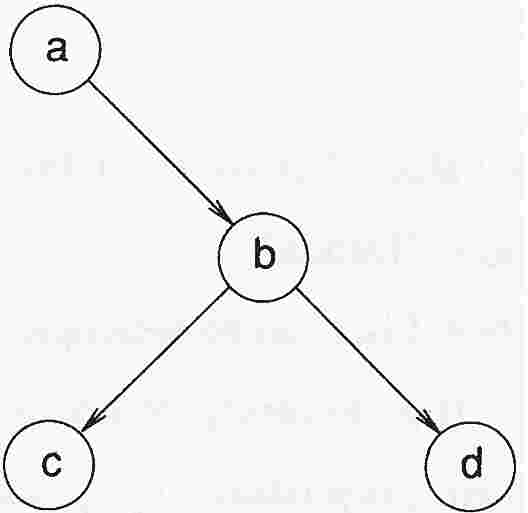
\includegraphics[width=1.8161in,height=1.7134in]{ib-img/ib-img002.jpg} 

Structures also can be used to represent loops, as in

{\ttfamily\mdseries
\ \ \ graph := [{\textquotedbl}a{\textquotedbl}, {\textquotedbl}{\textquotedbl}]\newline
 \ \ graph[2] := graph}

\noindent which can be depicted as

\ \  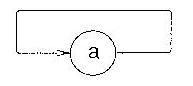
\includegraphics[width=1.4193in,height=0.5992in]{ib-img/ib-img003.jpg} 

Lists are not fixed in size. Elements can be added to them or removed
from them at their ends by queue and stack functions.

The function \texttt{put(a, x)} adds the value of \texttt{x} to the
right end of the increasing its size by one.  Similarly,
\texttt{push(a, x)} adds the value of \texttt{x} to the left end of
\texttt{a}. For example,

{\ttfamily\mdseries
\ \ \ lines := []\newline
 \ \ while put(lines, read(f))}

\noindent constructs a list of the lines from the file f. Conversely,

{\ttfamily\mdseries
\ \ \ lines := []\newline
 \ \ while push(lines, read(f))}

\noindent constructs a list of lines in reverse order.

The functions \texttt{pop(a)} and \texttt{get(a)} are the same. They
both remove an element from the left end of a and return it as the
value of the function call, but they fail if a is empty. Consequently,

{\ttfamily\mdseries
\ \ \ lines := []\newline
 \ \ while push(lines, read(f))\newline
 \ \ while write(pop(lines))}

\noindent writes out the lines of \texttt{f} in reverse order. The
function \texttt{pull(a)} is similar, but it removes an element from
the right end of \texttt{a}.

Other operations on lists include concatenation, which is denoted by

{\ttfamily\mdseries
\ \ \ a1 {\textbar}{\textbar}{\textbar} a2}

\noindent where \texttt{a1} and \texttt{a2} are lists. There is no
automatic conversion of other types to lists.

List sectioning is denoted by

{\ttfamily
\ \ \ a[i:j]}

The result is a \textit{new} list containing values \texttt{i} through
\texttt{j} of \texttt{a}.

There is no inherent limit to the size of a list, either when it is
originally created or as a result of adding elements to it.

{\sffamily\bfseries
2.1.6 Sets}

A set is an unordered collection of values. Unlike csets, which
contain only characters, sets are collections of Icon values that can
be of any type. A set is constructed from a list by
\texttt{set(a)}. For example,

{\ttfamily\mdseries
\ \ \ states := set([{\textquotedbl}Virginia{\textquotedbl}, {\textquotedbl}Rhode Island{\textquotedbl},
{\textquotedbl}Kansas{\textquotedbl}, \ \ \ \ \ \ \ \  \ {\textquotedbl}Illinois{\textquotedbl}])}

\noindent
assigns a set of four elements to \texttt{states}.

The operation

{\ttfamily\mdseries
\ \ \ member(s, x)}

\noindent
succeeds if the value of \texttt{x} is a member of \texttt{s} but
fails otherwise. The operation

{\ttfamily\mdseries
\ \ \ insert(s, x)}

\noindent
adds the value of \texttt{x} to \texttt{s} if it is not already a
member of \texttt{s}, while

{\ttfamily
\ \ \ delete(s, x)}

\noindent
deletes the value of \texttt{x} from \texttt{s}. The operations of
union, intersection, and difference for sets also are provided.

Like other structures, sets can be heterogeneous. A set can even be a
member of itself, as in

{\ttfamily\mdseries
\ \ \ insert(s, s)}

There is no contradiction here, since a set value is a pointer to the
structure for the set.

{\sffamily\bfseries
2.1.7 Tables}

A table is a set of pairs of values. Tables provide an associative
look mechanism as contrasted with positional references to lists. They
can be subscripted with an \textit{entry value }to which a value can
be assigned to make up a pair called a table element.

A table is created by

{\ttfamily\mdseries
\ \ \ table(x)}


Tables are empty initially. The value of x is an assigned default
value that is produced if the table is subscripted with an entry value
to which no value has been assigned (that is, for an element that is
not in the table). For example,

{\ttfamily\mdseries
\ \ \ states := table(0)}

\noindent assigns to states a table with a default value of 0. An
element can be added to states by an assignment such as

{\ttfamily\mdseries
\ \ \ states[{\textquotedbl}Oregon{\textquotedbl}] := 1}

\noindent which adds a table element for
\texttt{{\textquotedbl}Oregon{\textquotedbl}} with the value
\texttt{1} to \texttt{states}. On the other hand,

{\ttfamily\mdseries
\ \ \ write(states [{\textquotedbl}Utah{\textquotedbl}])}

\noindent writes \texttt{0}, the default value, if there is no element
in the table for \texttt{{\textquotedbl}Utah{\textquotedbl}}.

Tables can be heterogeneous and have a mixture of types for entry and
assigned values. Tables grow automatically in size as new elements are
added and there is no inherent limit on the size of a table.

{\sffamily\bfseries
2.1.8 Records}

A record is an aggregate of values that is referenced by named
fields. Each record type has a separate name. A record type and the
names of its fields are given in a declaration. For example,

{\ttfamily\mdseries
\ \ \ record rational(numerator, denominator)}

\noindent
declares a record of type rational with two fields: numerator and denominator.

An instance of a record is created by calling a record-constructor
function corresponding to the form of the declaration for the record
type. Thus,

{\ttfamily\mdseries
\ \ \ r := rational(3,5)}

\noindent
assigns to \texttt{r} a record of type rational with a
numerator field of 3 and a denominator field of 5. Fields are
referenced by name, as in

{\ttfamily\mdseries
\ \ \ write(r.numerator)}

\noindent which writes 3. Fields can also be referred to by position;
\texttt{r[1]} is equivalent to \texttt{r.numerator}.

There is no inherent limit to the number of different record
types. The same field names can be given for different record types,
and such fields need not be in the same position for all such record
types.

{\sffamily\bfseries
2.1.9 Input and Output}

Input and output in Icon are sequential and comparatively simple. The
standard input, standard output, and standard error output files are
the values of \texttt{\&input}, \texttt{\&output}, and
\texttt{\&errout}, respectively. The function

{\ttfamily\mdseries
\ \ \ open(s1,s2)}

\noindent opens the file whose name is \texttt{s1} according to
options given by \texttt{s2} and produces a value of type file.
Typical options are \texttt{{\textquotedbl}r{\textquotedbl}} for
opening for reading and \texttt{{\textquotedbl}w{\textquotedbl}} for
opening for writing. The default is
\texttt{{\textquotedbl}r{\textquotedbl}}. For example,

{\ttfamily\mdseries
\ \ \ log := open({\textquotedbl}grade.log{\textquotedbl}, {\textquotedbl}w{\textquotedbl})}

\noindent assigns a value of type file to log, corresponding to the
data file grade.log, which is opened for writing. The function open
fails if the specified file cannot be opened according to the options
given. The function \texttt{close(f)} closes the file \texttt{f}.

The function \texttt{read(f)} reads a line from the file \texttt{f}
but fails if an end of file is encountered. The default is standard
input if \texttt{f} is omitted.

The result of

{\ttfamily\mdseries
\ \ \ write(x1,x2, ..., xn)}

\noindent depends on the types of x1, x2, ..., xn. Strings and types
convertible to strings are written, but if one of the arguments is a
file, subsequent strings are written to that file. The default file is
standard output. Thus,

{\ttfamily\mdseries
\ \ \ write(s1,s2)}

\noindent
writes the concatenation of \texttt{s1} and \texttt{s2} to standard output, but

{\ttfamily\mdseries
\ \ \ write(log,s)}

\noindent
writes \texttt{s} to the file grade.log. In any event, write returns
the string value of the last argument written.

The function

{\ttfamily\mdseries
\ \ \ stop(x1, x2, ..., xn)}

\noindent
produces the same output as write, but it then terminates program execution.

{\sffamily\bfseries
2.1.10 Procedures}

\textbf{Procedure Declarations.} The executable portions of an Icon
program are contained in procedure declarations.  Program execution
begins with a call of the procedure main.

An example of a procedure declaration is:

{\ttfamily\mdseries
\ \ \ procedure maxstr(slist)\newline
 \ \ \ \ \ local max, value\newline
 \ \ \ \ \ max := 0\newline
 \ \ \ \ \ every value := *!slist do\newline
 \ \ \ \ \ \ \ \ if value{\textgreater} max then max := value\newline
 \ \ \ \ \ return max\newline
 \ \ end}


This procedure computes the longest string in a list of strings. The
formal parameter slist and the identifiers max and value are local to
calls of the procedure \texttt{maxstr()}. Storage for them is
allocated when \texttt{maxstr()} is called and deallocated when
\texttt{maxstr()} returns.

A procedure call has the same form as a function call. For example,

{\ttfamily\mdseries
\ \ \ lines := []\newline
 \ \ while put(lines, read(f))\newline
 \ \ write(maxstr(lines))}

\noindent
writes the length of the longest line in the file \texttt{f}.

A procedure call may fail to produce a result in the same way that a
built-in operation can fail. This is indicated by fail in the
procedure body in place of return. For example, the following
procedure returns the length of the longest string in \texttt{slist}
but fails if that length is less than limit:

{\ttfamily\mdseries
\ \ \ procedure maxstr(slist, limit)\newline
 \ \ \ \ \ local max, value\newline
 \ \ \ \ \ max := 0\newline
 \ \ \ \ \ every value := *!slist do\newline
 \ \ \ \ \ \ \ \ if value{\textgreater} max then max := value\newline
 \ \ \ \ \ if max {\textless} limit then fail else return max\newline
 \ \ end}

Flowing off the end of a procedure body without an explicit return is
equivalent to fail.

A procedure declaration may have static identifiers that are known
only to calls of that procedure but whose values are not destroyed
when a call returns. A procedure declaration also may have an initial
clause whose expression is evaluated only the first time the procedure
is called. The use of a static identifier and an initial clause is
illustrated by the following procedure, which returns the longest of
all the strings in the lists it has processed:

{\ttfamily\mdseries
\ \ \ procedure maxstrall(slist)\newline
 \ \ \ \ \ local value\newline
 \ \ \ \ \ static max\newline
 \ \ \ \ \ initial max := 0\newline
 \ \ \ \ \ every value := *!slist do\newline
 \ \ \ \ \ \ \ \ if value{\textgreater} max then max := value\newline
 \ \ \ \ \ return max\newline
 \ \ end}

\textbf{Procedures and Functions.} Procedures and functions are used
in the same way. Their names have global scope.  Other identifiers can
be declared to have global scope, as in

{\ttfamily\mdseries
\ \ \ global count}

Such global declarations are on a par with procedure declarations and
cannot occur within procedure declarations.

A call such as

{\ttfamily\mdseries
\ \ \ write(maxstr(lines))}

\noindent
applies the \textit{value} of the identifier \texttt{maxstr} to
\texttt{lines} and applies the \textit{value} of the identifier
\texttt{write} to the result. There is nothing fixed about the values
of such identifiers. In this case, the initial value of
\texttt{maxstr} is a procedure, as a consequence of the procedure
declaration for it. Similarly, the initial value of \texttt{write} is
a function. These values can be assigned to other variables, as in

{\ttfamily\mdseries
\ \ \ print := write\newline
 \ \ \ \ \ \ \ \ \ \ ...\newline
 \ \ \textrm{print(maxstr(lines))}}

\noindent in which the function that is the initial value of
\texttt{write} is assigned to \texttt{print}.

Similarly, nothing prevents an assignment to an identifier whose
initial value is a procedure. Consequently,

{\ttfamily\mdseries
\ \ \ write := 3}

\noindent
assigns an integer to \texttt{write}, replacing its initial function value.

Although it is typical to call a procedure by using an identifier that
has the procedure value, the procedure used in a call can be
computed. The general form of a call is

{\ttfamily\mdseries
\textit{\ \ \ expr}\textit{\TextSubscript{0}}\textit{(expr}\textit{\TextSubscript{1}}\textit{,
expr}\textit{\TextSubscript{2}}\textit{, }..., \textit{expr}\textit{\TextSubscript{n}}\textit{)}}

\noindent where the value of
\textit{expr\TextSubscript{0}} is applied to the
arguments resulting from the evaluation of
\textit{expr\TextSubscript{1}}
\textit{expr\TextSubscript{2}}, ...,
\textit{expr\TextSubscript{n}}. For example,

{\ttfamily\mdseries
\ \ \ (proclist[i])\textit{(expr\TextSubscript{1}}, ,
\textit{expr\TextSubscript{2}},
..., \textit{expr\TextSubscript{n})}}

\noindent
applies the procedure that is the \texttt{i}th element of \texttt{proclist}.

Procedures may be called recursively. The recursive nature of a call
depends on the fact that procedure names are global. The
{\textquotedbl}Fibonacci strings{\textquotedbl} provide an example:

{\ttfamily\mdseries
\ \ \ procedure fibstr(i)\newline
 \ \ \ \ \ if i = 1 then return {\textquotedbl}a{\textquotedbl}\newline
 \ \ \ \ \ else if i = 2 then return {\textquotedbl}b{\textquotedbl}\newline
 \ \ \ \ \ else return fibstr(i - 1) {\textbar}{\textbar} fibstr(i - 2)\newline
 \ \ end}

An identifier that is not declared in a procedure and is not global
defaults to local. Thus, local declarations can be omitted, as in

{\ttfamily\mdseries
\ \ \ procedure maxstr(slist)\newline
 \ \ \ \ \ max := 0\newline
 \ \ \ \ \ every value := * !slist do\newline
 \ \ \ \ \ \ \ \ if value {\textgreater} max then max := value\newline
 \ \ \ \ \ return max\newline
 \ \ end}


\textbf{Procedures as Generators}. In addition to returning and
failing, a procedure can also suspend. In this case, the values of its
arguments and local identifiers are not destroyed, and the call can
be resumed to produce another result in the same way a built-in
generator can be resumed. An example of such a generator is

{\ttfamily\mdseries
\ \ \ procedure intseq(i)\newline
 \ \ \ \ \ repeat \{\newline
 \ \ \ \ \ \ \ \ suspend i\newline
 \ \ \ \ \ \ \ \ i +:= 1\newline
 \ \ \ \ \ \ \ \ \}\newline
 \ \ end}

A call \texttt{intseq(10)}, for example, is capable of generating the
infinite sequence of integers 10, 11, 12, ... .  For example,

{\ttfamily\mdseries
\ \ \ every f(intseq(10) {\textbackslash} 5)}

\noindent
calls f(10), f(11), f(12), f(13), and f(14).

If the argument of suspend is a generator, the generator is resumed
when the call is resumed and the call suspends again with the result
it produces. A generator of the Fibonacci strings provides an example:

\ \ \ procedure fibstrseq()\newline
 \ \ \ \ \ local s1, s2, s3\newline
 \ \ \ \ \ s1 := {\textquotedbl}a{\textquotedbl}\newline
 \ \ \ \ \ s2 := {\textquotedbl}b{\textquotedbl}\newline
 \ \ \ \ \ suspend (s1 {\textbar} s2)\newline
 \ \ \ \ \ repeat \{\newline
 \ \ \ \ \ \ \ \ suspend s3 := s1 {\textbar}{\textbar} s2\newline
 \ \ \ \ \ \ \ \ s1 := s2\newline
 \ \ \ \ \ \ \ \ s2 := s3\newline
 \ \ \ \ \ \ \ \ \}\newline
 \ \ end

When this procedure is called, the first suspend expression produces
the value of\ \ s1, {\textquotedbl}a{\textquotedbl}. If the call of
\texttt{fibstrseq()} is resumed, the argument of \texttt{suspend} is
resumed and produces the value of \texttt{s2},
\texttt{{\textquotedbl}b{\textquotedbl}}. If the call is resumed
again, there is no further result for the first \texttt{suspend}, and
evaluation continues to the \texttt{repeat} loop.

Repeated alternation often is useful in supplying an endless number of
alternatives. For example, the procedure \texttt{intseq(i)} can be
rewritten as

{\ttfamily\mdseries
\ \ \ procedure intseq(i)\newline
 \ \ \ \ \ suspend i {\textbar} (i +:= {\textbar}1)\newline
 \ \ end}

Note that \texttt{{\textbar}1} is used to provide an endless sequence
of increments.


\textbf{Argument Transmission}. Omitted arguments in a procedure or
function call (including trailing ones) default to the null
value. Extra arguments are evaluated, but their values are discarded.

Some functions, such as \texttt{write()}, may be called with an
arbitrary number of arguments. All arguments to procedures and
functions are passed by value. If the evaluation of an argument
expression fails, the procedure or function is not called. This
applies to extra arguments. Arguments are not dereferenced until all
of them have been evaluated. Dereferencing cannot fail. Since no
argument is dereferenced until all argument expressions are evaluated,
expressions with side effects can produce unexpected results. Thus, in

{\ttfamily\mdseries
\ \ \ write(s, s := {\textquotedbl}hello{\textquotedbl})}

\noindent the value written is \texttt{hellohello}, regardless of the
value of \texttt{s} before the evaluation of the second argument of
\texttt{write()}.


\textbf{Dereferencing in Return Expressions}. The result returned from
a procedure call is dereferenced unless it is a global identifier, a
static identifier, a subscripted structure, or a subscripted
string-valued global identifier.

In these exceptional cases, the variable is returned and assignment
can be made to the procedure call. An example is

{\ttfamily\mdseries
\ \ \ procedure maxel(a, i, j)\newline
 \ \ \ \ \ if i {\textgreater} j then return a[i]\newline
 \ \ \ \ \ else return a[j]\newline
 \ \ end}

Here a list element, depending on the values of \texttt{i} and
\texttt{j}, is returned. An assignment can be made to it, as in

{\ttfamily\mdseries
\ \ \ maxel(lines, i, j) := {\textquotedbl}end{\textquotedbl}}

\noindent which assigns \texttt{{\textquotedbl}end{\textquotedbl}} to
\texttt{lines[i]} or \texttt{lines[j]}, depending on the values of
\texttt{i} and \texttt{j}.


\textbf{Mutual Evaluation}. In a call expression, the value of
\textit{expr}\textit{\TextSubscript{0}} can be an integer
\texttt{i} as well as a procedure. In this case, called
\textit{mutual evaluation}, the result of the \texttt{i}th
argument is produced. For example,

{\ttfamily\mdseries
\ \ \ i := 1(find(s1, line1), find(s2, line2))}

\noindent assigns to \texttt{i} the position of \texttt{s1} in
\texttt{line1}, provided \texttt{s1} occurs in \texttt{line1} and that
\texttt{s2} occurs in line2. If either call of find fails, the
expression fails and no assignment is made.

The selection integer in mutual evaluation can be negative, in which
case it is interpreted relative to the end of the argument
list. Consequently,

{\ttfamily\mdseries
\textit{\ \ \ (-1)(expr\TextSubscript{1}},\textit{expr\TextSubscript{2}}\textit{, }...,
\textit{expr\TextSubscript{n}}\textit{)}}

\noindent
produces the result of \textit{expr\TextSubscript{n}} and is equivalent to


\textit{\ \ \ expr1 }\& \textit{expr2 }\& ... \& \textit{exprn}

The selection integer can be omitted, in which case it defaults to -1.


{\sffamily\bfseries
2.1.11 Co-Expressions}

The evaluation of an expression in Icon is limited to the site in the
program where it appears. Its results can be produced only at that
site as a result of iteration or goal-directed evaluation. For
example, the results generated by \texttt{intseq(i)} described in
Section 2.1.10 can only be produced where it is called, as in

{\ttfamily\mdseries
\ \ \ every f(intseq(10) {\textbackslash} 5)}

It is often useful, however, to be able to produce the results of a
generator at various places in the program as the need for them
arises. Co-expressions provide this facility by giving a context for
the evaluation of an expression that is maintained in a data
structure. Co-expressions can be \textit{activated }to produce the
results of a generator on demand, at any time and place in the
program.

A co-expression is constructed by

\ \ \ create \textit{expr}

The expression \textit{expr} is not evaluated at this time. Instead,
an object is produced through which \textit{expr} can be resumed at a
later time. For example,

{\ttfamily\mdseries
\ \ \ label := create ({\textquotedbl}L{\textquotedbl} {\textbar}{\textbar} (1 to 100) {\textbar}{\textbar}
{\textquotedbl}:{\textquotedbl})}

\noindent assigns to label a co-expression for the expression

{\ttfamily\mdseries
\ \ \ {\textquotedbl}L{\textquotedbl} {\textbar}{\textbar} (1 to 100) {\textbar}{\textbar}
{\textquotedbl}:{\textquotedbl}}

The operation \texttt{@label} activates this co-expression, which
corresponds to resuming its expression. For example,

{\ttfamily\mdseries
\ \ \ write(@label)\newline
 \ \ write({\textquotedbl} \ \ \ tstl \ \ \ \ count{\textquotedbl})\newline
 \ \ write(@label)}

\noindent
writes

{\ttfamily\mdseries
\ \ \ L1:\newline
 \ \ \ \ \ \ \ tstl \ \ \ \ count\newline
 \ \ L2:}

If the resumption of the expression in a co-expression does not
produce a result, the co-expression activation fails.  For example,
after \texttt{@label} has been evaluated 100 times, subsequent
evaluations of \texttt{@label} fail. The number of results that a
co-expression \texttt{e} has produced is given by \texttt{*e}.

The general form of the activation expression is

\textit{\ \ \ expr1 }@ \textit{expr2}

\noindent which activates \textit{expr2} and transmits the result of
\textit{expr1} to it. This form of activation can be used to return a
result to the co-expression that activated the current one.

A co-expression is a value like any other value in Icon and can be
passed as an argument to a procedure, returned from a procedure. and
so forth. A co-expression can survive the call of the procedure in
which it is created.

If the argument of a create expression contains identifiers that are
local to the procedure in which the create occurs, copies of these
local identifiers are included in the co-expression with the values
they have at the time the create expression is evaluated. These copied
identifiers subsequently are independent of the local identifiers in
the procedure. Consider, for example,

{\ttfamily\mdseries
\ \ \ procedure labgen(tag)\newline
 \ \ \ \ \ local i, j\newline
\ \  ...\newline
\ \  i := 10\newline
\ \  j := 20\newline
\ \  e := create (tag {\textbar}{\textbar} (i to j) {\textbar}{\textbar} {\textquotedbl}:{\textquotedbl})\newline
\ \  ...\newline
\ \  i := j\newline
\ \  if i {\textgreater} 15 then return e\newline
\ \  ...\newline
 \ \ end}

The expression

{\ttfamily\mdseries
\ \ \ labels := labgen({\textquotedbl}X{\textquotedbl})}

\noindent assigns to labels a co-expression that is equivalent to evaluating

{\ttfamily\mdseries
\ \ \ create ({\textquotedbl}X{\textquotedbl} {\textbar}{\textbar} (10 to 20) {\textbar}{\textbar}
{\textquotedbl}:{\textquotedbl})}

The fact that \texttt{i} is changed after the co-expression was
assigned to \texttt{e}, but before \texttt{e} returns, does not affect
the co-expression, since it contains copies of \texttt{i} and
\texttt{j} at the time it was created.  Subsequent changes to the
values of \texttt{i} or \texttt{j} do not affect the co-expression.

A copy of a co-expression \texttt{e} is produced by the
\textit{refresh }operation, \texttt{\^{}e}. When a refreshed copy of a
co-expression is made, its expression is reset to its initial state,
and the values of any local identifiers in it are reset to the values
they had when the co-expression was created. For example,

{\ttfamily\mdseries
\ \ \ newlabels := \^{}labels}

\noindent assigns to \texttt{newlabels} a co-expression that is
capable of producing the same results as labels, regardless of whether
or not labels has been activated.

The value of the keyword \texttt{\&main} is the co-expression for the
call of \texttt{main()} that initiates program execution.


{\sffamily\bfseries
2.1.12 Diagnostic Facilities}

\textbf{String Images}. The function \texttt{type(x)} only produces
the string name of the type of \texttt{x}, but the function
\texttt{image(x)} produces a string that shows the value of
\texttt{x}. For strings and csets, the value is shown with surrounding
quotation marks in the fashion of program literals. For example,

{\ttfamily\mdseries
\ \ \ write(image({\textquotedbl}Hi there!{\textquotedbl}))}

\noindent writes \texttt{{\textquotedbl}Hi there!{\textquotedbl}}, while

{\ttfamily\mdseries
\ \ \ write(image('aeiou'))}

\noindent writes \texttt{{}'aeiou'}.

For structures, the type name and size are given. For example,

{\ttfamily\mdseries
\ \ \ write(image([]))}

\noindent writes \texttt{list(0)}.

Various forms are used for other types of data, using type names where
necessary so that different types of values are distinguishable.


\textbf{Tracing}. If the value of the keyword \texttt{\&trace} is
nonzero, a trace message is produced whenever a procedure is called,
returns, fails, suspends, or is resumed. Trace messages are written to
standard error output. The value of \texttt{\&trace} is decremented
for every trace message. Tracing stops if the value of
\texttt{\&trace} becomes zero, which is its initial value. Suppose
that the following program is contained in the file fibstr.icn:

{\ttfamily\mdseries
\ \ \ procedure main()\newline
 \ \ \ \ \ \&trace := -1\newline
 \ \ \ \ \ fibstr(3)\newline
 \ \ end\newline
\newline
 \ \ procedure fibstr(i)\newline
 \ \ \ \ \ if i = 1 then return {\textquotedbl}a{\textquotedbl}\newline
 \ \ \ \ \ else if i = 2 then return {\textquotedbl}b{\textquotedbl}\newline
 \ \ \ \ \ else return fibstr(i -1) {\textbar}{\textbar} fibstr(i -2)\newline
 \ \ end}

The trace output of this program is

{\ttfamily\mdseries
\textrm{\ \ \ fibstr.icn: 3\ \ {\textbar} fibstr(3)}\newline
 \ \ fibstr.icn: 9\ \ {\textbar} {\textbar} fibstr(2)\newline
 \ \ fibstr.icn: 8\ \ {\textbar} {\textbar} fibstr returned {\textquotedbl}b{\textquotedbl}\newline
 \ \ fibstr .icn: 9\ \ {\textbar} {\textbar} fibstr(1)\newline
 \ \ fibstr.icn: 7\ \ {\textbar} {\textbar} fibstr returned {\textquotedbl}b{\textquotedbl}\newline
 \ \ fibstr.icn: 9\ \ {\textbar} fibstr returned {\textquotedbl}ba{\textquotedbl}\newline
 \ \ fibstr.icn: 4\ \ main failed}

In addition to the indentation corresponding to the level of procedure
call, the value of the keyword \texttt{\&level} also is the current
level of call.

\textbf{Displaying Identifier Values}. The function
\texttt{display(i,f)} writes a list of all identifiers and their
values for \texttt{i} levels of procedure calls, starting at the
current level. If \texttt{i} is omitted, the default is
\texttt{\&level}, while if \texttt{f} is omitted, the list is written
to standard error output. The format of the listing produced by
display is illustrated by the following program:

{\ttfamily
\ \ \ procedure main()\newline
 \ \ \ \ \ log := open({\textquotedbl}grade.log{\textquotedbl}, {\textquotedbl}w{\textquotedbl})\newline
 \ \ \ \ \ while write(log, check(readO))\newline
 \ \ end}


\bigskip

{\ttfamily
\ \ \ procedure check(value)\newline
 \ \ \ \ \ static count\newline
 \ \ \ \ \ initial count := 0\newline
 \ \ \ \ \ if numeric(value) then \{\newline
 \ \ \ \ \ \ \ \ count +:= 1\newline
 \ \ \ \ \ \ \ \ return value\newline
 \ \ \ \ \ \ \ \ \}\newline
 \ \ \ \ \ else \{\newline
 \ \ \ \ \ \ \ \ display()\newline
 \ \ \ \ \ \ \ \ stop({\textquotedbl}nonnumeric value{\textquotedbl})\newline
 \ \ \ \ \ \ \ \ \}\newline
 \ \ end}


Suppose that the tenth line of input is the nonnumeric string
\texttt{{\textquotedbl}3.a{\textquotedbl}}. Then the output of
\texttt{display()} is

{\ttfamily\mdseries
\ \ \ check local identifiers:\newline
 \ \ \ \ \ value = {\textquotedbl}3.a{\textquotedbl}\newline
 \ \ \ \ \ count = 9\newline
 \ \ main local identifiers:\newline
 \ \ \ \ \ log = file(grade.log)\newline
 \ \ global identifiers:\newline
 \ \ \ \ \ main = procedure main\newline
 \ \ \ \ \ check = procedure check\newline
 \ \ \ \ \ open = function open\newline
 \ \ \ \ \ write = function write\newline
 \ \ \ \ \ read = function read\newline
 \ \ \ \ \ numeric = function numeric\newline
 \ \ \ \ \ display = function display\newline
 \ \ \ \ \ stop = function stop}


\textbf{Error Messages}. If an error is encountered during program
execution, a message is written to standard error output and execution
is terminated. For example, if the tenth line of a program contained
in the file check.icn is

{\ttfamily\mdseries
\ \ \ i +:= {\textquotedbl}x{\textquotedbl}}

\noindent
evaluation of this expression produces the error message

{\ttfamily\mdseries
\ \ \ Run-time error 102 at line 10 in check.icn\newline
 \ \ numeric expected\newline
 \ \ offending value: {\textquotedbl}x{\textquotedbl}}


\section{Language Features and the Implementation}

Even a cursory consideration of Icon reveals that some of its features
present implementation problems and require approaches that are
different from ones used in more conventional languages. In the case
of a language of the size and complexity of Icon, it is important to
place different aspects of the implementation in perspective and to
identify specific problems.


\textbf{Values and Variables.} The absence of type declarations in
Icon has far-reaching implications. Since any variable may have a
value of any type and the type may change from time to time during
program execution, there must be a way of representing values
uniformly. This is a significant challenge in a language with a wide
variety of types ranging from integers to
co-expressions. Heterogeneous structures follow as a natural
consequence of the lack of type declarations.

In one sense, the absence of type declarations simplifies the
implementation: there is not much that can be done about types during
program translation (compilation), and some of the work that is
normally performed by conventional compilers can be avoided. The
problems do not go away, however -- they just move to another part of
the implementation, since run-time type checking is
required. Automatic type conversion according to context goes
hand-in-hand with type checking.


\textbf{Storage Management.} Since strings and structures are created
during program execution, rather than being declared, the space for
them must be allocated as needed at run time. This implies, in turn,
some mechanism for reclaiming space that has been allocated but which
is no longer needed--{\textquotedbl}garbage collection.{\textquotedbl}
These issues are complicated by the diversity of types and sizes of
objects, the lack of any inherent size limitations, and the
possibility of pointer loops in circular structures.


\textbf{Strings.} Independent of storage-management considerations,
strings require special attention in the implementation. The emphasis
of Icon is on string processing, and it is necessary to be able to
process large amounts of string data sufficiently. Strings may be very
long and many operations produce substrings of other strings. The
repertoire of string analysis and string synthesis functions is
large. All this adds up to the need for a well-designed and coherent
mechanism for handling strings.


\textbf{Structures.} Icon's unusual structures, with sophisticated
access mechanisms, also pose problems. In particular, structures that
can change in size and can grow without limit require different
implementation approaches than static structures of fixed size and
organization.


The flexibility of positional, stack, and queue access mechanisms for
lists requires compromises to balance efficient access for different
uses. Sets of values with arbitrary types, combined with a range of
set operations, pose non-trivial implementation problems. Tables are
similar to sets, but require additional attention because of the
implicit way that elements are added.


\textbf{Procedures and Functions.} Since procedures and functions are
values, they must be represented as data objects.  More significantly,
the meaning of a function call cannot, in general, be determined when
a program is translated. The expression write(s) may write a string or
it may do something else, depending on whether or not write still has
its initial value. Such meanings must, instead, be determined at run
time.


\textbf{Polymorphic Operations.} Although the meanings of operations
cannot be changed during program execution in the way that the
meanings of calls can, several operations perform different
computations depending on the types of their operands. Thus, x[i] may
subscript a string, a list, or a table.

The meanings of some operations also depend on whether they occur in
an assignment or a dereferencing context. For example, if s has a
string value, assignment to s [i] is an abbreviation for a
concatenation followed by an assignment to s, while if s[i] occurs in
a context where its value is needed, it is simply a substring
operation. Moreover, the context cannot, in general, be determined at
translation time.

The way subscripting operations are specified in Icon offers
considerable convenience to the programmer at the expense of
considerable problems for the implementer.


\textbf{Expression Evaluation.} Generators and goal-directed
evaluation present obvious implementation problems. There is a large
body of knowledge about the implementation of expression evaluation
for conventional languages in which expressions always produce a
single result, but there is comparatively little knowledge about
implementing expressions that produce results in sequence.

While there are languages in which expressions can produce more than
one result, this capability is limited to specific contexts, such as
pattern matching, or to specific control structures or data objects.

In Icon, generators and goal-directed evaluation are general and
pervasive and apply to all evaluation contexts and to all types of
data. Consequently, their implementation requires a fresh
approach. The mechanism also has to handle the use of failure to drive
control structures and must support novel control structures, such as
alternation and limitation. Efficiency is a serious concern, since
whatever mechanism is used to implement generators is also used in
conventional computational situations in which only one result is
needed.


\textbf{String Scanning.} String scanning is comparatively simple. The
subject and position --- {\textquotedbl}state variables{\textquotedbl}
--- have to be saved at the beginning of string scanning and restored
when it is completed.  Actual string analysis and matching follow
trivially from generators and goal-directed evaluation.


\textbf{Co-Expressions.} Co-expressions, which are only relevant
because of the expression-evaluation mechanism of Icon, introduce a
whole new set of complexities. Without co-expressions, the results
that a generator can produce are limited to its site in the
program. Control backtracking is limited syntactically, and its scope
can be determined during program translation. With co-expressions, a
generator in a state of suspension can be activated at any place and
time during program execution.


\textsc{Retrospective}: Icon has a number of unusual features that are
designed to facilitate programming, and it has an extensive repertoire
of string and structure operations. One of Icon's notable
characteristics is the freedom from translation-time constraints and
the ability to specify and change the meanings of operations at run
time. This run-time flexibility is valuable to the programmer, but it
places substantial burdens on the implementation---and also makes it
interesting.

At the top level, there is the question of how actually to carry out
some of the more sophisticated operations. Then there are questions of
efficiency, both in execution speed and storage utilization. There are
endless possibilities for alternative approaches and refinements.

It is worth noting that many aspects of the implementation are
relatively independent of each other and can be approached
separately. Operations on strings and structures are largely disjoint
and can, except for general considerations of the representation of
values and storage management, be treated as independent problems.

The independence of expression evaluation from other implementation
considerations is even clearer. Without generators and goal-directed
evaluation, Icon would be a fairly conventional high-level string and
structure processing language, albeit one with interesting
implementation problems. On the other hand, generators and
goal-directed evaluation are not dependent in any significant way on
string and structure data types. Generators, goal-directed evaluation,
and related control structures could just as well be incorporated in a
programming language emphasizing numerical computation. The
implementation problems related to expression evaluation in the two
contexts are largely the same.

While untyped variables and automatic storage management have
pervasive effects on the overall implementation of Icon, there are
several aspects of Icon that are separable from the rest of the
language and its implementation. Any specific data structure, string
scanning, or co-expressions could be eliminated from the language
without significantly affecting the rest of the
implementation. Similarly, new data structures and new access
mechanisms could be added without requiring significant modifications
to the balance of the implementation.

{\sffamily\bfseries
EXERCISES}

\liststyleLi
\begin{enumerate}
\item \begin{enumerate}
\item 
\ What is the outcome of the following expression if the file f contains a line consisting of
{\textquotedbl}end{\textquotedbl}, or if it does not?\newline
 \ \ \ \ while line := read(f) do\newline
 \ \ \ \ \ \ \ \ \ if line == {\textquotedbl}end{\textquotedbl} then break\newline
 \ \ \ \ \ \ \ \ \ else write(line)
\item 
\ What does\newline
 \ \ \ \ \ write({\textquotedbl}hello{\textquotedbl} {\textbar} {\textquotedbl}howdy{\textquotedbl})\newline
write?
\item 
\ What is the result of evaluating the following expression:\newline
\texttt{ \ \ \ \ \ 1(1 to 3) {\textgreater} 10}
\item 
\ Explain the rationale for dereferencing of variables when a procedure call returns.
\item 
\ Give an example of a situation in which it cannot be determined until run time whether a string subscripting
expression is used in an assignment or a dereferencing context.
\end{enumerate}
\end{enumerate}
